% THIS IS SIGPROC-SP.TEX - VERSION 3.0
% WORKS WITH V3.1SP OF ACM_PROC_ARTICLE-SP.CLS
% JUNE 2007
%
% It is an example file showing how to use the 'acm_proc_article-sp.cls' V3.1SP
% LaTeX2e document class file for Conference Proceedings submissions.
% ----------------------------------------------------------------------------------------------------------------
% This .tex file (and associated .cls V3.1SP) *DOES NOT* produce:
%       1) The Permission Statement
%       2) The Conference (location) Info information
%       3) The Copyright Line with ACM data
%       4) Page numbering
% ---------------------------------------------------------------------------------------------------------------
% It is an example which *does* use the .bib file (from which the .bbl file
% is produced).
% REMEMBER HOWEVER: After having produced the .bbl file,
% and prior to final submission,
% you need to 'insert'  your .bbl file into your source .tex file so as to provide
% ONE 'self-contained' source file.
%
% Questions regarding SIGS should be sent to
% Adrienne Griscti ---> griscti@acm.org
%
% Questions/suggestions regarding the guidelines, .tex and .cls files, etc. to
% Gerald Murray ---> murray@acm.org
%
% For tracking purposes - this is V3.0SP - JUNE 2007

\documentclass{acm_proc_article-sp}
%\usepackage[latin1]{inputenc}
%\usepackage[spanish]{babel}
\begin{document}

\title{Computaci\'on Gr\'afica - A jugar al sapo!}
%
% You need the command \numberofauthors to handle the 'placement
% and alignment' of the authors beneath the title.
%
% For aesthetic reasons, we recommend 'three authors at a time'
% i.e. three 'name/affiliation blocks' be placed beneath the title.
%
% NOTE: You are NOT restricted in how many 'rows' of
% "name/affiliations" may appear. We just ask that you restrict
% the number of 'columns' to three.
%
% Because of the available 'opening page real-estate'
% we ask you to refrain from putting more than six authors
% (two rows with three columns) beneath the article title.
% More than six makes the first-page appear very cluttered indeed.
%
% Use the \alignauthor commands to handle the names
% and affiliations for an 'aesthetic maximum' of six authors.
% Add names, affiliations, addresses for
% the seventh etc. author(s) as the argument for the
% \additionalauthors command.
% These 'additional authors' will be output/set for you
% without further effort on your part as the last section in
% the body of your article BEFORE References or any Appendices.

\numberofauthors{1} %  in this sample file, there are a *total*
% of EIGHT authors. SIX appear on the 'first-page' (for formatting
% reasons) and the remaining two appear in the \additionalauthors section.
%
\author{
% You can go ahead and credit any number of authors here,
% e.g. one 'row of three' or two rows (consisting of one row of three
% and a second row of one, two or three).
%
% The command \alignauthor (no curly braces needed) should
% precede each author name, affiliation/snail-mail address and
% e-mail address. Additionally, tag each line of
% affiliation/address with \affaddr, and tag the
% e-mail address with \email.
%
% 1st. author
\alignauthor Nicol\'as D\'iaz Pa\'is\\
       \affaddr{Instituto Tecnol\'ogico de Buenos Aires}\\
	\affaddr{Buenos Aires, Argentina}\\
       \email{ndiazpai@alu.itba.edu.ar}}


\maketitle
\begin{abstract}
En este art\'iculo, se detallan los aspectos, implementaci\'on, dise\~no y experiencias en el desarrollo del juego del Sapo. Dicho juego, 
se desarroll\'o para la materia Computaci\'on Gr\'afica, del ITBA, en el lenguaje de programaci\'on Java. La totalidad del trabajo se desarroll\'o con herramientas 
\textit{open source} y 
por ende conserva dicho esp\'iritu.
\end{abstract}

\keywords{Computaci\'on Gr\'afica, Juego, Java, JME, Juego del Sapo}

\section{Introducci\'on}
\label{sec:introduccion}

Si bien su origen sigue siendo incierto, algunos atribuyen la aparicion de este juego a la civilizaci\'on Inca. Los pobladores ten\'ian por costumbre arrojar monedas a los lagos y, seg\'un la leyenda, si los sapos en dicho momento se tragaban la moneda, se le cumplir\'ia un deseo a la persona que la hab\'ia arrojado.
Lo cierto es que este juego se hizo muy popular en varios pa\'ises, y se pueden encontrar una diversidad enorme en los muebles
utilizados para el mismo, algunos m\'as completos que otros. Un ejemplo se muestra en la figura \ref{fig:sapoReal}.


\begin{figure}[!ht]
	\centering
		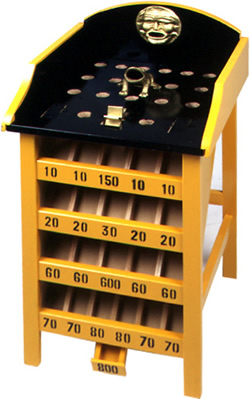
\includegraphics[]{img/juegoSapo.jpg}
	\caption{Juego del Sapo}
	\label{fig:sapoReal}
\end{figure}


\subsection{Reglamento}
\label{subsec:reg}
Las reglas del juego son muy sencillas: los jugadores arrojan monedas al mueble acondicionado para el juego (de aqu\'i en adelante, se lo llamar\'a simplemente "Sapo") y dependiendo en el agujero donde cae la moneda, se otorgan los puntos. De los agujeros se extiende una canaleta hasta los dep\'ositos, donde est\'an indicados los valores. El mayor puntaje se obtiene cuando la moneda cae en el agujero del sapo propiamente indicado. 
La distancia a la cual el jugador se para delante del Sapo influye en la dificultad del juego. Naturalmente, el jugador puede optar por correrse a la izquiera o derecha de la caja, y obtener de esa forma un \'angulo de tiro que le resulte m\'as c\'omodo.

En la figura \ref{fig:sapoGame} se muestra una pantalla del juego desarrollado.

\begin{figure}[!ht]
	\centering
		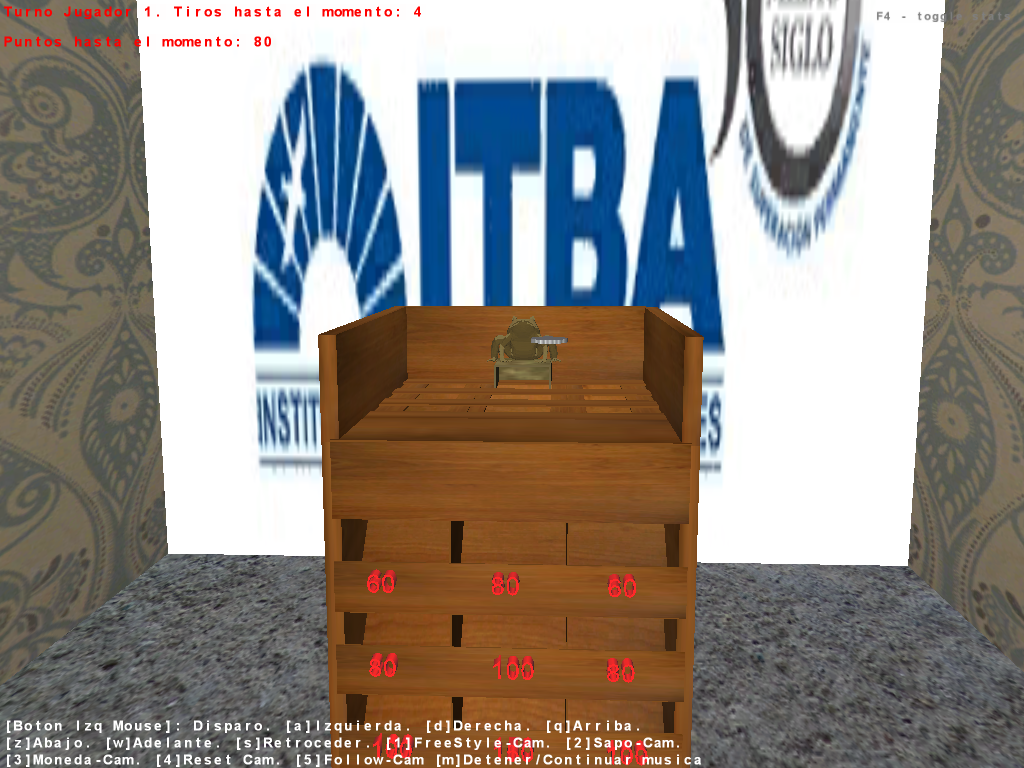
\includegraphics[width=8cm,height=6.45cm]{img/simpleShoot.png}
	\caption{Captura del Juego desarrollado.}
	\label{fig:sapoGame}
\end{figure}


\section{Detalles de Implementaci\'on}
\label{sec:impl}

En esta secci\'on se detallan los aspectos m\'as importantes de la implementaci\'on del juego.
\subsection{Framework utilizado}

El framework utilizado para resolver la f\'isica y creaci\'on de la escena (rasterizaci\'on) fue el JMonkeyEngine [R01]. Se trata de un framework muy completo en los temas antes mencionados, y permite centrarse en la grafica, modelado, jugabilidad y desarrollo del juego, dejando la f\'isica a cargo de JMonkey. Si bien cuenta con una version estable, su desarrollo continua en el presente y presenta algunos problemas que no fueron solucionados por sus desarrolladores. 

\subsection{Modelado de la escena}

El modelado de la escena constituye la parte central del trabajo. Gracias a la utilizaci\'on del framework, los aspectos de jugabilidad y f\'isica pueden resolverse con la ayuda de JMonkey, pero el modelado de la escena, es el mayor problema a enfrentar en el desarrollo de este juego. 
Para ello, mediante las primitivas ofrecidas por el framework, se dise\~no el Sapo como lo har\'ia un carpintero: primero, las cajas exteriores, luego, las canaletas internas, la tapa y por ultimo detalles como el sapo decorativo. El trabajo en el dise\~no del mueble, casi art\'istico, se hizo mediante el seguimiento de los planos pensados con  anterioridad y consumi\'o la mayor parte del tiempo. El plano del corte de secci\'on utilizado en la diagramaci\'on del sapo se observa en la figura \ref{fig:sapoSection}.

Para la construcci\'on de la escena, se utiliza un archivo XML conteniendo la informaci\'on y medidas de los elementos que la componen. De esta forma se logra una interface de f\'acil acceso y modificaci\'on si as\'i lo requiriere, sin la necesidad de compilar de nuevo la aplicaci\'on.

\begin{figure}[!ht]
	\centering
		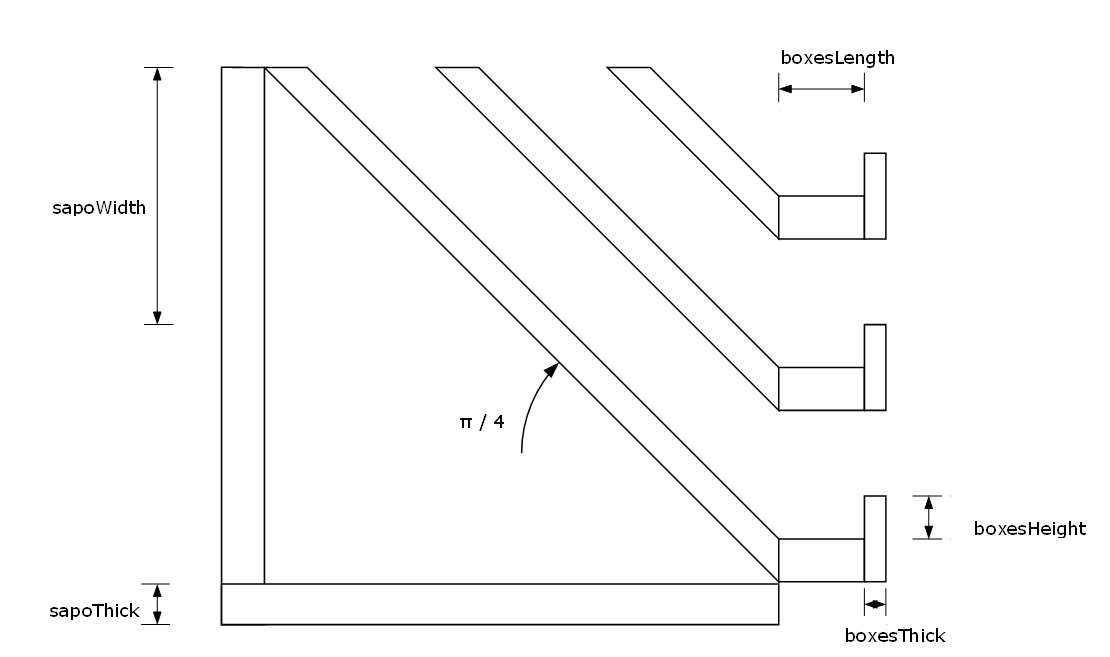
\includegraphics[width=9cm,height=6.45cm]{img/sapoLayout.png}
	\caption{Plano del corte de secci\'on.}
	\label{fig:sapoSection}
\end{figure}


\subsection{Jugador}
\label{impl:jugador}

Inspirado en los juegos \textit{first-person-shooter}\footnote{Juegos en primera persona. Por ejemplo, el juego desarrollado por 
la empresa Sierra, \textit{Counter Strike}}, se decidi\'o ubicar al jugador en primera persona. Para ello, la camara muestra lo 
que ve el jugador, y a donde apunta el disparo, pudiendo variar la altura, la distancia, el \'angulo de tiro y hasta inclusive 
la potencia del disparo.

\subsection{Camaras}
\label{impl:camaras}

Ofreciendole al jugador un poder \'unico de visualizaci\'on, se implementaron varios tipos de c\'amaras en el transcurso del juego. El jugador puede elegir aquella c\'amara que le resulte m\'as c\'omoda. Las posibles c\'amaras son:

\begin{enumerate}
\item \textbf{FreeStyle-Cam:} C\'amara libre en visualizaci\'on y movimiento, inclusive despues del disparo. \\
\item \textbf{Sapo-Cam:} C\'amara fija en el sapo del juego, y siempre enfocada a la moneda. \\
\item \textbf{Moneda-Cam:} C\'amara fija en la moneda, que permite seguir el transcurso de la misma. \\
\item \textbf{Follow-Cam:} C\'amara siempre enfocada a la moneda desde el lugar del disparo, una vez que ya se ha efectuado. \\
\end{enumerate}


\subsection{Texturas y sonidos}

En pos de entregar una mayor sensaci\'on de realismo y placer al jugador, se implementaron texturas en todos los objetos y musica durante la construcci\'on del juego. En la figura \ref{fig:texturas} se muestra una vista cercana al Sapo, donde se aprecia las texturas utilizadas para la construcci\'on del mismo y otros elementos, como la moneda. Se tuvo especial cuidado en la elecci\'on de estos elementos, para no sobrecargar de manera significativa la renderizaci\'on y actualizaci\'on de cada \textit{frame}. 

\begin{figure}[!ht]
	\centering
		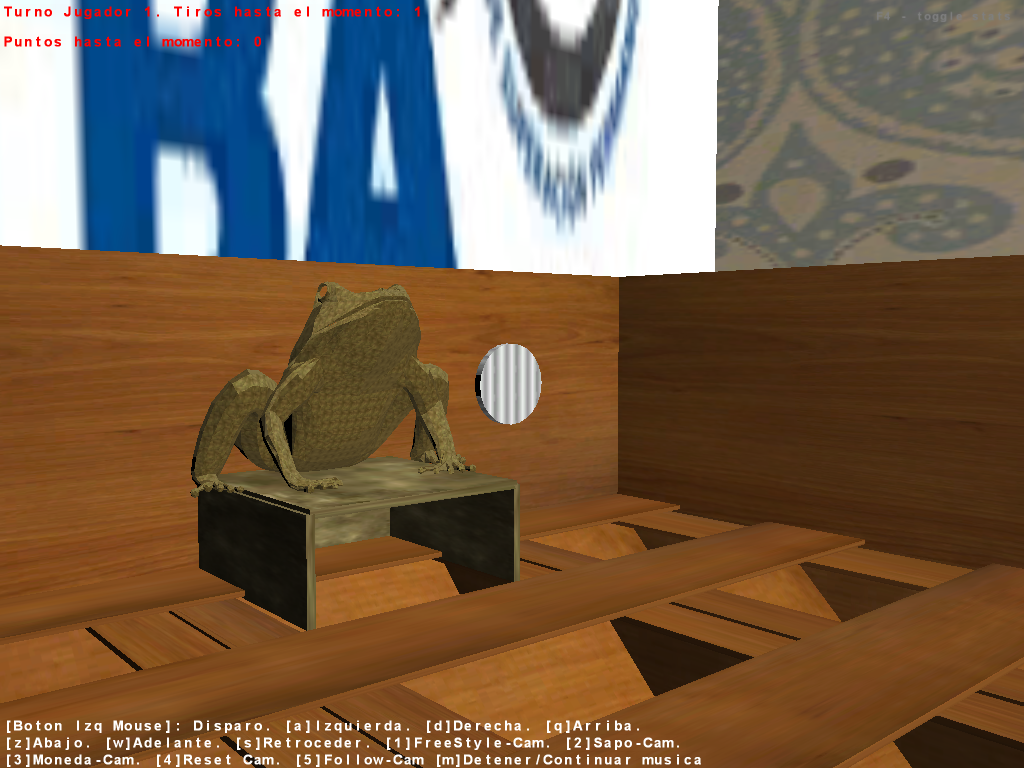
\includegraphics[width=8cm,height=6.45cm]{img/littleSapoShoot.png}
	\caption{Texturas.}
	\label{fig:texturas}
\end{figure}

\section{El juego}
\label{sec:juego}

En esta secci\'on se explican los detalles a tener en cuenta para la ejecuci\'on del mismo y la forma de jugar.
\subsection{Ejecucion}
Una de las caracter\'isticas m\'as importantes de este desarrollo, es que puede ejecutarse en varias plataformas. En esta entrega se muestra c\'omo ejecutar el juego tanto en entornos Windows como en GNU\textbackslash Linux, en arquitecturas de 32 o 64 bits \footnote{Aunque en esta entrega solo se pens\'o en los ambientes mencionados, se pueden conseguir las bibliotecas nativas para correr el juego en otros entornos, como Mac o Solaris}.
Los pasos de ejecuci\'on se detallan a continuaci\'on:

\begin{itemize}
 \item \textbf{Windows:} Simplemente, ejecutar el archivo sapoGame.bat. El unico requisito es contar con la maquina virtual de java instalada previamente.
\item \textbf{Linux:} Ejecutar el script sapoGame.sh (seteando previamente permisos de ejecuci\'on).
\item \textbf{Otros ambientes:} Ejecutar con la maquina virtual de Java el archivo sapoGame.jar, seteando previamente en el library path la ubicaci\'on de las bibliotecas nativas correspondientes.
\end{itemize}
 

\subsection{Forma de jugar}
Como se menciona en la secci\'on \ref{impl:jugador}, el juego tiene por modalidad el uso de primera persona. Con el mouse, se establece el angulo de tiro (tanto vertical como horizontal) y una vez establecido, mediante el bot\'on izquierdo, se procede a hacer el disparo. El tiempo que se mantiene presionado el bot\'on establece la potencia de disparo, donde a mayor tiempo se traduce en mayor fuerza con la que ser\'a arrojada la moneda. La moneda disparada impacta con los diversos objetos de la escena, produciendo rebotes y ca\'idas, hasta quedar totalmente detenida. En ese momento, se informa al jugador el puntaje obtenido y lo habilita a realizar un nuevo tiro (hasta que la moneda no se detenga, no se permite relizar otro disparo). Ejemplo de esto \'ultimo, se observa en la figura \ref{fig:sapoHit}. Luego de 10 tiros, se cambia de turno al segundo jugador. Finalizado el juego, se muestra el resultado de la partida y se ofrece reiniciar el juego mediante la tecla de barra espaciadora.

Tambien se ofrece la posibilidad de moverse hacia adelante, mediante la tecla "w" del teclado y retroceder con la tecla "s". De esta manera se ajusta la distancia del jugador al Sapo. Mediante las teclas "a" y "d" se produce pasos a la izquierda y derecha respectivamente, modificando el angulo de visi\'on (y consecuentemente de tiro) del jugador.
Si el jugador decide cambiar la altura del disparo, basta con presionar las teclas "q" y "z" para ubicarse a una altura mayor o menor, respectivamente. En la figura \ref{fig:farSapo} se aprecia la vista de un jugador, donde se ha variado la altura, angulo y distancia del disparo.


Para poder cambiar las c\'amaras, explicadas en la secci\'on \ref{impl:camaras}, se utilizan las siguientes teclas num\'ericas:
\begin{enumerate}
 \item FreeStyle-Cam
 \item Sapo-Cam
 \item Moneda-Cam 
 \item Resetea la posici\'on de la c\'amara
 \item Follow-Cam 
\end{enumerate}

Por \'ultimo, para poder detener o reiniciar la m\'usica del juego, se utiliza la tecla "m". 

\begin{figure}[!ht]
	\centering
		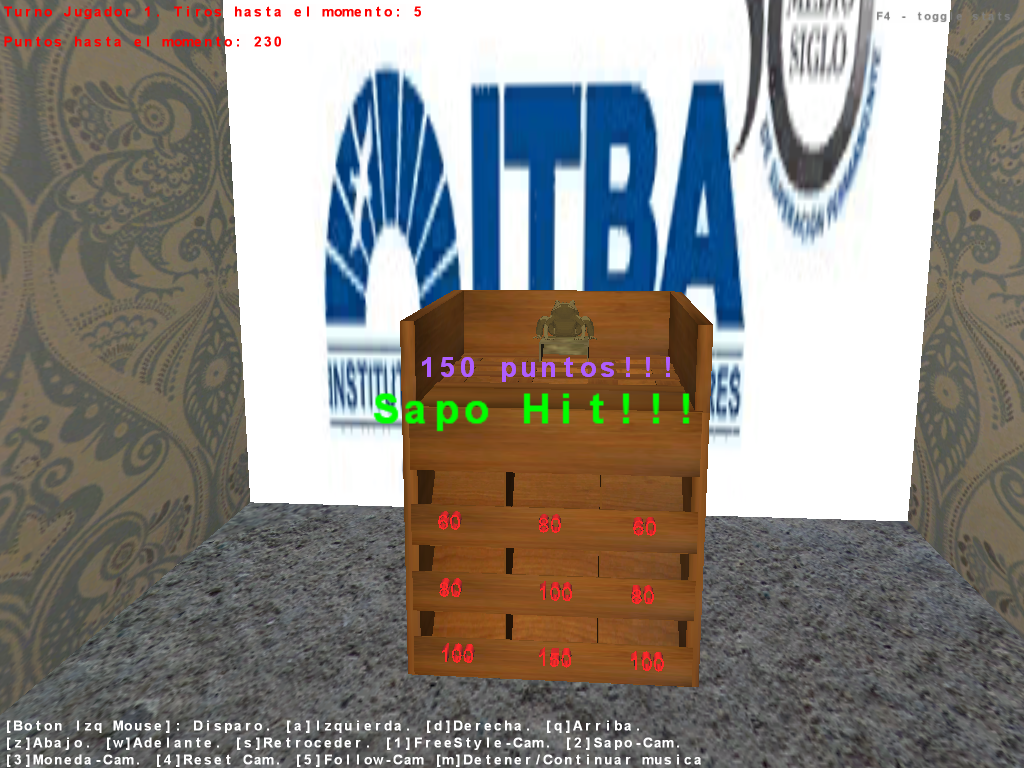
\includegraphics[width=8cm,height=6.45cm]{img/sapoShoot.png}
	\caption{Disparo acertado al agujero del sapo.}
	\label{fig:sapoHit}
\end{figure}


\begin{figure}[!ht]
	\centering
		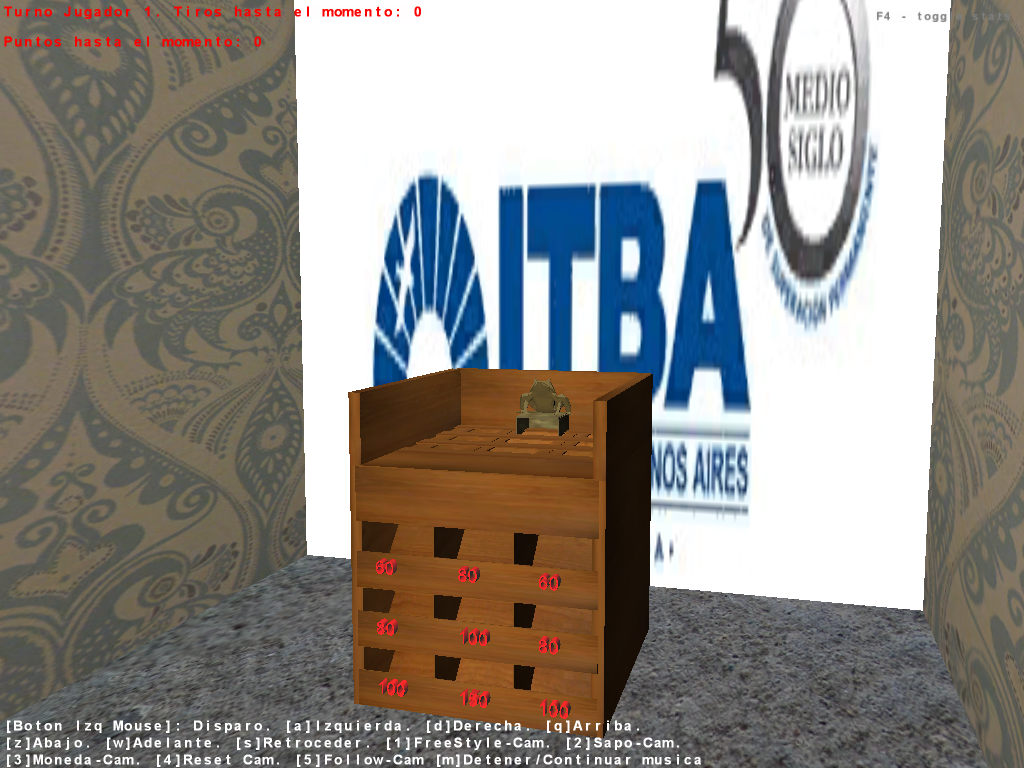
\includegraphics[width=8cm,height=6.45cm]{img/perspSapo.png}
	\caption{El juego desde otra posicion.}
	\label{fig:farSapo}
\end{figure}

\section{Experiencias en el desarrollo}

\subsection{Problemas Encontrados}

La mayor fuente de problemas se encontraron en el modelado de la escena y las limitaciones contenidas en el framework.

Con respecto al modelado, poder lograr un mueble lo m\'as fiel a los comunmente vistos, es un trabajo delicado y costoso. Sin embargo, algunas caracter\'isticas fueron imposibles de realizar debido a las limitaciones del framework. Entre ellas, se ubican la de poder importar modelos realizados con otros programas \footnote{Por ejemplo, Blender o MeshLab, ambos open source.} pero sin preservar la geometr\'ia. Por lo tanto, no puede desarrollarse el agujero en la boca del sapo o el dispositivo de rueda. 

Otra de las limitaciones, se encuentra en las primitivas ofrecidas por el framework para el modelado. No es posible lograr agujeros circulares, ya que s\'i se producen visualmente, pero no se refleja en la generaci\'on de la f\'isica correspondiente. Se contact\'o a los desarrolladores del framework para superar esta limitaci\'on, pero sugirieron tenerlo en cuenta para las pr\'oximas releases del framework, no ofreciendolo hasta el momento.

\subsection{Posibles mejoras}

Un modelado un poco m\'as sofisticado incluir\'ia tramas diagonales sobre la tapa, de forma tal de lograr agujeros octogonales, y no cuadrados. 
Otra posible mejora, se encuentra en la interface, mostrando informaci\'on de la ubicaci\'on del jugador y barra de potencia del disparo.

\section{Conclusiones}
Una de las conclusiones m\'as importantes a resaltar, consiste en la buena experiencia que consisti\'o el acercamiento hacia este tipo de desarrollo. Si bien el framework resuelve muchos aspectos en cuanto a la f\'isica, el planeamiento del juego requiri\'o un estudio intensivo previo del modelado de la caja del Sapo. 
Con respecto al framework, se concluye que cuenta con muchas ventajas. Es pr\'actico, potente, y f\'acil de usar. Sin embargo, las limitaciones que tiene son importantes y eso puede llegar a influir de forma considerable la implementaci\'on de cualquier juego. 



\section*{Referencias}

[R01] JMonkeyEngine - Java Framework http://www.jmonkeyengine.com/


% That's all folks!
\end{document}
